\begin{appendices}
	\crefalias{chapter}{appcha}
	\crefalias{section}{appsec}
	\renewcommand{\thesection}{\Alph{chapter}\arabic{section}}

	\chapter{Additional results from \cref{cha:obesity_genetic_signatures_and_cancer}}
	\label{app:a}

	\section{Comparison of the Creighton \textit{et al.} obesity metagene in standardised or non-standardised CR data}
	\label{sec:metagenes_created_from_raw_data_vs_standardised_data}

	\begin{figure}[htpb]
		\centering
		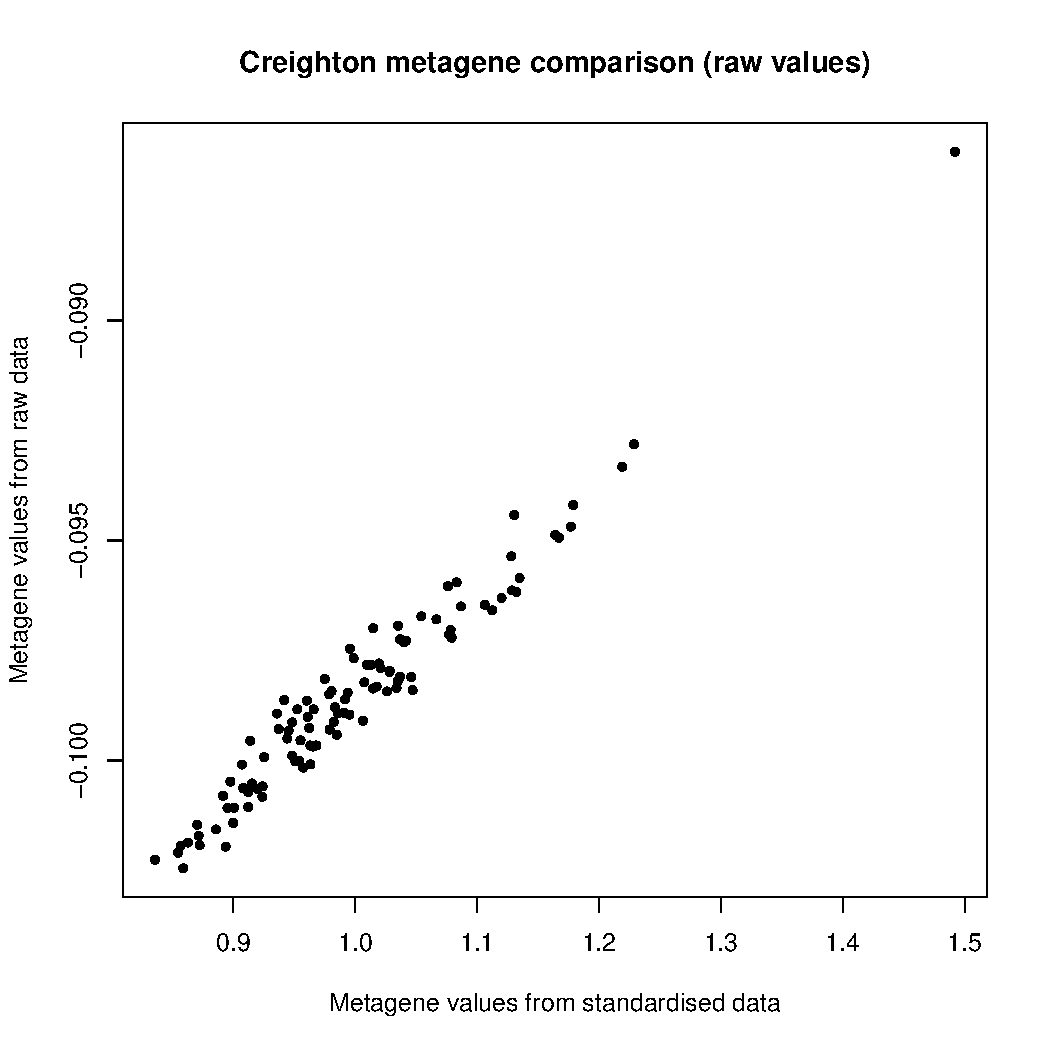
\includegraphics[width=0.45\linewidth,page=1]{appendix/check_raw_vs_std_mg}
		\hfill
		\includegraphics[width=0.45\linewidth,page=2]{appendix/check_raw_vs_std_mg}
		\caption[Comparison of the raw and ranked Creighton \textit{et al.} obesity metagene scores from the standardised or non-standardised CR data]{Scatter plots showing the raw and ranked Creighton \textit{et al.} obesity metagene scores from the standardised or non-standardised CR data.
		The \gls{rma}-normalised CR data was standardised or used as is to generate the obesity metagene scores.
		The metagene scores were ranked based on the number of samples in the CR data set.
		}
		\label{fig:appendix/check_raw_vs_std}
	\end{figure}

	\section{Comparison of the Creighton \textit{et al.} obesity metagene in standardised or non-standardised \gls{icgc} data}
	\label{sec:comp_cr_raw_std_icgc}

	As shown in \cref{fig:appendix/check_raw_vs_std}, the Creighton \textit{et al.} obesity metagene values generated from the transformation matrices (from standardised or non-standardised CR data) were more consistent (or less variable) in the standardised \gls{icgc} \gls{blca} data, compared with the non-standardised data.
	Results from \cref{fig:appendix/check_raw_vs_std_tm} suggested that there was no obvious difference in the quality of the metagenes generated from standardised or non-standardised TM.
	Only the results from \gls{blca} data set are shown, as the results from the other \gls{icgc} cancer types showed very similar results.

	\begin{figure}[h]
		\centering
		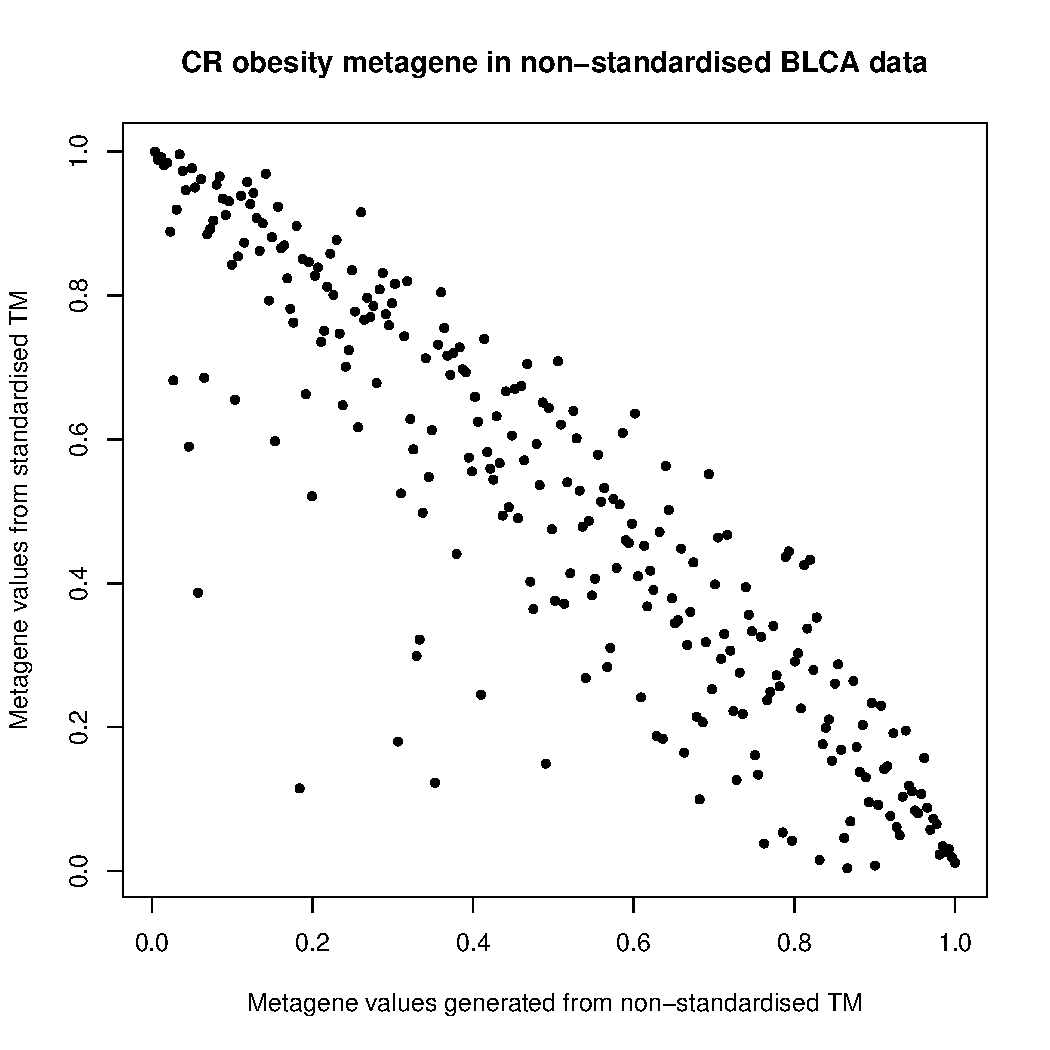
\includegraphics[width=0.45\linewidth,page=1]{appendix/crtcga_raw_vs_std}
		\hfill
		\includegraphics[width=0.45\linewidth,page=2]{appendix/crtcga_raw_vs_std}\\
		\caption[Comparison of the Creighton \textit{et al.} obesity metagene generated from the standardised or non-standardised TM]{Scatter plots comparing the Creighton \textit{et al.} obesity metagene generated from the transformation matrix (from standardised or non-standardised CR data) in the non-standardised (left) and standardised (right) \gls{icgc} \gls{blca} data.}
		\label{fig:appendix/check_raw_vs_std}
	\end{figure}

	\begin{figure}[h]
		\centering
		\includegraphics[width=0.45\linewidth,page=3]{appendix/crtcga_raw_vs_std}
		\hfill
		\includegraphics[width=0.45\linewidth,page=4]{appendix/crtcga_raw_vs_std}\\
		\caption[Comparison of the Creighton \textit{et al.} obesity metagene generated from the standardised or non-standardised  \gls{icgc} \gls{blca} data]{Scatter plots comparing the Creighton \textit{et al.} obesity metagene from the non-standardised  and standardised  \gls{icgc} \gls{blca} data, generated by the application of the transformation matrix from the non-standardised (left) or standardised (right) CR data.}
		\label{fig:appendix/check_raw_vs_std_tm}
	\end{figure}

	\section{Remainder of the results of FM obesity metagenes in the \gls{icgc} cancer data sets}
	\label{sec:rest_of_the_fm_icgc_cancer_heatmap_results}

	\cref{fig:appendix/fm_ob_meta_heatmap_icgc} shows the association of the FM obesity metagene with the gene expression pattern of the FM obesity associated genetic signature in the other \gls{icgc} cancer data sets.
	\cref{fig:appendix/fm_ob_meta_box_scatter_icgc} shows the association of the FM obesity metagene scores with the patient \gls{bmi} and \gls{bmi} status.
	Clearly, the FM metagene was able to capture the overall gene expression patterns, but was not significantly associated with the patient \gls{bmi} or \gls{bmi} status.

	\begin{figure}[htpb]
		\centering
		\includegraphics[width=0.32\linewidth,page=8]{appendix/fm_meta_ICGC}\\
		\includegraphics[width=0.32\linewidth,page=13]{appendix/fm_meta_ICGC}
		\includegraphics[width=0.32\linewidth,page=18]{appendix/fm_meta_ICGC}
		\includegraphics[width=0.32\linewidth,page=23]{appendix/fm_meta_ICGC}\\
		\includegraphics[width=0.32\linewidth,page=28]{appendix/fm_meta_ICGC}
		\includegraphics[width=0.32\linewidth,page=33]{appendix/fm_meta_ICGC}
		\includegraphics[width=0.32\linewidth,page=38]{appendix/fm_meta_ICGC}\\
		\caption[Association of the FM obesity metagene with the sample gene expressions in the other \gls{icgc} data]{Heatmaps showing the association of the FM obesity metagenes  with the sample gene expressions in the other \gls{icgc} data sets.
		Scales are as described in previous figures.}
		\label{fig:appendix/fm_ob_meta_heatmap_icgc}
	\end{figure}

	\begin{figure}[htpb]
		\centering
		\includegraphics[page=9,width=0.42\linewidth]{appendix/fm_meta_ICGC}
		\hfill
		\includegraphics[page=10,width=0.42\linewidth]{appendix/fm_meta_ICGC}\\
		\caption[Association of the FM obesity metagene with the patient \gls{bmi}/\gls{bmi} status in the other \gls{icgc} data]{Box plots and scatter plots showing the association of the FM obesity metagene with the patient \gls{bmi} status  and \gls{bmi}, respectively, in the \gls{icgc} data sets.
		P-values and $R^2$-value are as described in previous figures.}
		\label{fig:appendix/fm_ob_meta_box_scatter_icgc}
	\end{figure}

	\begin{figure}[htpb]
		\ContinuedFloat
		\captionsetup{list=off,format=cont}
		\centering
		\includegraphics[page=14,width=0.45\linewidth]{appendix/fm_meta_ICGC}
		\hfill
		\includegraphics[page=15,width=0.45\linewidth]{appendix/fm_meta_ICGC}\\
		\includegraphics[page=19,width=0.45\linewidth]{appendix/fm_meta_ICGC}
		\hfill
		\includegraphics[page=20,width=0.45\linewidth]{appendix/fm_meta_ICGC}\\
		\includegraphics[page=24,width=0.45\linewidth]{appendix/fm_meta_ICGC}
		\hfill
		\includegraphics[page=25,width=0.45\linewidth]{appendix/fm_meta_ICGC}\\
		\caption{Name}
	\end{figure}

	\begin{figure}[htpb]
		\ContinuedFloat
		\captionsetup{list=off,format=cont}
		\centering
		\includegraphics[page=29,width=0.45\linewidth]{appendix/fm_meta_ICGC}
		\hfill
		\includegraphics[page=30,width=0.45\linewidth]{appendix/fm_meta_ICGC}\\
		\includegraphics[page=34,width=0.45\linewidth]{appendix/fm_meta_ICGC}
		\hfill
		\includegraphics[page=35,width=0.45\linewidth]{appendix/fm_meta_ICGC}\\
		\includegraphics[page=39,width=0.45\linewidth]{appendix/fm_meta_ICGC}
		\hfill
		\includegraphics[page=40,width=0.45\linewidth]{appendix/fm_meta_ICGC}\\
		\caption{Name}
	\end{figure}

	\section{Direction of all the obesity metagenes from the CR data}
	\label{sec:direction_of_all_the_obesity_metagenes_from_the_cr_data}

	The direction of the obesity metagenes identified from the CR data were examined and corrected for (\cref{fig:crob_meta_direction}).
	Gene probes that were common to all obesity associated genetic signatures were used to examine whether the metagene was in the correct direction, relative to the other obesity metagenes

	\begin{figure}[htpb]
		\centering
		\includegraphics[width=0.32\linewidth,page=3]{appendix/cr_meta_direction_raw}
		\includegraphics[width=0.32\linewidth,page=6]{appendix/cr_meta_direction_raw}\\
		\includegraphics[width=0.32\linewidth,page=9]{appendix/cr_meta_direction_raw}
		\includegraphics[width=0.32\linewidth,page=12]{appendix/cr_meta_direction_raw}
		\includegraphics[width=0.32\linewidth,page=15]{appendix/cr_meta_direction_raw}\\
		\includegraphics[width=0.32\linewidth,page=18]{appendix/cr_meta_direction_raw}
		\includegraphics[width=0.32\linewidth,page=21]{appendix/cr_meta_direction_raw}
		\includegraphics[width=0.32\linewidth,page=24]{appendix/cr_meta_direction_raw}\\
		\caption[Directionality of the obesity metagenes in the CR data]{Heatmaps showing the gene expression of the obesity associated genetic signatures with the obesity metagene in \gls{rma}-normalised CR data set.
		The gene probes that were common to all of the obesity associated genetic signatures were used to determine the direction of the obesity metagenes.
		The scales and axes are the same as the previous heatmaps.
		}
		\label{fig:crob_meta_direction}
	\end{figure}

	\section{Remainder of the results of the other CR obesity metagenes in \gls{nzbc} data set}
	\label{sec:rest_of_the_cr_ob_meta_heatmap_results_cris}

	All of the other obesity metagenes from the CR data set were able to capture the overall gene expressions of the samples in the \gls{nzbc} data set (\cref{fig:appendix/cr_ob_meta_heatmap_cris}).
	However, none of the CR obesity metagenes were able to significantly associate with the sample \gls{bmi}/\gls{bmi} status in the \gls{nzbc} data set (\cref{fig:appendix/cr_ob_meta_box_scatter_cris}).

	\begin{figure}[htp!]
		\centering
		\includegraphics[width=0.32\linewidth,page=8]{appendix/cris_crdeg_trans_meta}\\
		\includegraphics[width=0.32\linewidth,page=13]{appendix/cris_crdeg_trans_meta}
		\includegraphics[width=0.32\linewidth,page=18]{appendix/cris_crdeg_trans_meta}
		\includegraphics[width=0.32\linewidth,page=23]{appendix/cris_crdeg_trans_meta}\\
		\includegraphics[width=0.32\linewidth,page=28]{appendix/cris_crdeg_trans_meta}
		\includegraphics[width=0.32\linewidth,page=33]{appendix/cris_crdeg_trans_meta}
		\includegraphics[width=0.32\linewidth,page=38]{appendix/cris_crdeg_trans_meta}\\
		\caption[Association of the other CR obesity metagenes with the sample gene expressions in the \gls{nzbc} data]{Heatmaps showing the association of the other obesity metagenes identified from the CR data with the sample gene expressions from the \gls{nzbc} data set.
		Scales are as described in previous figures.}
		\label{fig:appendix/cr_ob_meta_heatmap_cris}
	\end{figure}

	\begin{figure}[htpb]
		\centering
		\includegraphics[page=9,width=0.42\linewidth]{appendix/cris_crdeg_trans_meta}
		\hfill
		\includegraphics[page=10,width=0.42\linewidth]{appendix/cris_crdeg_trans_meta}\\
		\caption[Association of the other CR obesity metagenes with the sample \gls{bmi}/\gls{bmi} status in the \gls{nzbc} data]{Box plots and scatter plots showing the association of the other CR obesity metagenes with the sample \gls{bmi} status  and \gls{bmi} from the \gls{nzbc} data set, respectively.
		P-values and $R^2$-value are as described in previous figures.}
		\label{fig:appendix/cr_ob_meta_box_scatter_cris}
	\end{figure}

	\begin{figure}[htpb]
		\ContinuedFloat
		\captionsetup{list=off,format=cont}
		\centering
		\includegraphics[page=14,width=0.45\linewidth]{appendix/cris_crdeg_trans_meta}
		\hfill
		\includegraphics[page=15,width=0.45\linewidth]{appendix/cris_crdeg_trans_meta}\\
		\includegraphics[page=19,width=0.45\linewidth]{appendix/cris_crdeg_trans_meta}
		\hfill
		\includegraphics[page=20,width=0.45\linewidth]{appendix/cris_crdeg_trans_meta}\\
		\includegraphics[page=24,width=0.45\linewidth]{appendix/cris_crdeg_trans_meta}
		\hfill
		\includegraphics[page=25,width=0.45\linewidth]{appendix/cris_crdeg_trans_meta}\\
		\caption{Name}
	\end{figure}

	\begin{figure}[htpb]
		\ContinuedFloat
		\captionsetup{list=off,format=cont}
		\centering
		\includegraphics[page=29,width=0.45\linewidth]{appendix/cris_crdeg_trans_meta}
		\hfill
		\includegraphics[page=30,width=0.45\linewidth]{appendix/cris_crdeg_trans_meta}\\
		\includegraphics[page=34,width=0.45\linewidth]{appendix/cris_crdeg_trans_meta}
		\hfill
		\includegraphics[page=35,width=0.45\linewidth]{appendix/cris_crdeg_trans_meta}\\
		\includegraphics[page=39,width=0.45\linewidth]{appendix/cris_crdeg_trans_meta}
		\hfill
		\includegraphics[page=40,width=0.45\linewidth]{appendix/cris_crdeg_trans_meta}\\
		\caption{Name}
	\end{figure}

	\section{Remainder of the results of the other Creighton \textit{et al.} obesity metagenes in the \gls{icgc} cancer data sets}
	\label{sec:rest_of_the_cr_icgc_cancer_heatmap_results}

	As shown in \cref{fig:appendix/cr_icgc_heatmap}, the original obesity metagene from the Creighton \textit{et al.} study was reflective of the sample gene expression levels of the obesity associated genetic signature in all of the other \gls{icgc} cancer data sets.
	However, none of the \gls{icgc} cancer data sets (other than the \gls{blca} data set; \cref{fig:crmetaicgc} in \cref{sec:creighton_obesity_metagene}) showed any significant association of the sample \gls{bmi} or \gls{bmi} status with the Or obesity metagene (\cref{fig:appendix/cr_icgc_box_scatter}).
	The heatmaps, box plots and scatter plots for the other CR obesity metagenes in other \gls{icgc} cancer types are not shown, as many of the plots were very similar to the plots from the \gls{blca} data set.
	The statistics from the results of the box and scatter plots in the other \gls{icgc} cancer types were summarised in \cref{tab:degmetacesc,tab:degmetacoad,tab:degmetakirp,tab:degmetalihc,tab:degmetaread,tab:degmetaskcm,tab:degmetaucec}.

	\begin{figure}[htp!]
		\centering
		\includegraphics[width=0.32\linewidth,page=8]{appendix/crtcga_std}\\
		\vspace{1em}
		\includegraphics[width=0.32\linewidth,page=13]{appendix/crtcga_std}
		\includegraphics[width=0.32\linewidth,page=18]{appendix/crtcga_std}
		\includegraphics[width=0.32\linewidth,page=23]{appendix/crtcga_std}\\
		\vspace{1em}
		\includegraphics[width=0.32\linewidth,page=28]{appendix/crtcga_std}
		\includegraphics[width=0.32\linewidth,page=33]{appendix/crtcga_std}
		\includegraphics[width=0.32\linewidth,page=38]{appendix/crtcga_std}\\
		\caption[Obesity metagene from the \citet{Creighton2012} study and the sample gene expressions in the other \gls{icgc} cancer types]{Heatmaps showing the association of obesity metagene from the \citet{Creighton2012} study with sample gene expression from the other \gls{icgc} data sets.
		Level of expression is represented in the top right histogram, where low and high gene expression were colour-coded with blue and red, respectively.
		Each row of the heatmap represents a gene from the obesity associated genetic signature, and each column of the heatmap represents a sample from the \gls{icgc} data.
		The obesity associated metagene scores of the samples are shown in a separate row at top of the heatmap, and the tree diagram of the heirarchical clustering of the genes is shown to the left of the heatmap. }
		\label{fig:appendix/cr_icgc_heatmap}
	\end{figure}

	\begin{figure}[htpb]
		\centering
		\includegraphics[page=9,width=0.45\linewidth]{appendix/crtcga_std}
		\hfill
		\includegraphics[page=10,width=0.45\linewidth]{appendix/crtcga_std}\\
		\includegraphics[page=14,width=0.45\linewidth]{appendix/crtcga_std}
		\hfill
		\includegraphics[page=15,width=0.45\linewidth]{appendix/crtcga_std}\\
		\caption[Obesity metagene from the \citet{Creighton2012} study and the sample \gls{bmi}/\gls{bmi} status in the other \gls{icgc} cancer types]{Box plots and scatter plots showing the association of obesity metagene from the \citet{Creighton2012} study with the sample \gls{bmi} status  and \gls{bmi} from the other \gls{icgc} data sets, respectively.
		In the box plot, the p-values above the groups represent the statistical significance of the association of the metagene with the overweight or obese group compared with the normal weight group.
		The \gls{anova} p-value shows the statistical significance of the association of the metagene with the sample \gls{bmi} groups.
		In the scatter plot, $R^2$- and p-values describe the adjusted coefficient of determination of the regression line and the statistical significance of the linear model used to draw the regression line, respectively.}
		\label{fig:appendix/cr_icgc_box_scatter}
	\end{figure}

	\begin{figure}[htpb]
		\ContinuedFloat
		\captionsetup{list=off,format=cont}
		\centering
		\includegraphics[page=19,width=0.45\linewidth]{appendix/crtcga_std}
		\hfill
		\includegraphics[page=20,width=0.45\linewidth]{appendix/crtcga_std}\\
		\includegraphics[page=24,width=0.45\linewidth]{appendix/crtcga_std}
		\hfill
		\includegraphics[page=25,width=0.45\linewidth]{appendix/crtcga_std}\\
		\includegraphics[page=29,width=0.45\linewidth]{appendix/crtcga_std}
		\hfill
		\includegraphics[page=30,width=0.45\linewidth]{appendix/crtcga_std}\\
		\caption{Name}
	\end{figure}

	\begin{figure}[htpb]
		\ContinuedFloat
		\captionsetup{list=off,format=cont}
		\centering
		\includegraphics[page=34,width=0.45\linewidth]{appendix/crtcga_std}
		\hfill
		\includegraphics[page=35,width=0.45\linewidth]{appendix/crtcga_std}\\
		\includegraphics[page=39,width=0.45\linewidth]{appendix/crtcga_std}
		\hfill
		\includegraphics[page=40,width=0.45\linewidth]{appendix/crtcga_std}\\
		\caption{Name}
	\end{figure}

\begin{table}[htpb]
	\centering
	\caption[Statistics of all the obesity metagenes in the \gls{icgc} \acrshort{cesc} cancer data]{Statistics of all the obesity metagenes in the \gls{icgc} \gls{cesc} cancer data}
	\label{tab:degmetacesc}
	\begin{threeparttable}
		\begin{tabular}{lccccc}
			& \multicolumn{3}{c}{ P-values} & \multicolumn{2}{c}{ Regression line statistics}\\
			\cmidrule(r){2-4} \cmidrule(r){5-6}
			Metagenes &  Overweight &  Obese &  \gls{anova} &  R$^2$ &  P \\
			\hline
			\hline
			\rule{0pt}{2.25ex}Cr      & 0.9332                      & 0.5302  & 0.7622             & -0.003950  & 0.7265              \\
			Res     & 0.9205                      & 0.3369  & 0.6043             & 0.004249   & 0.8122              \\
			CrOl    & 0.8940                      & 0.1430  & 0.2959             & -0.0004927 & 0.3465              \\
			ResOl   & 0.9930                      & 0.1705  & 0.3078             & 0.003263   & 0.1898              \\
			Ca      & 0.8861                      & 0.3616  & 0.6426             & -0.003307  & 0.6073              \\
			CaRes   & 0.8323                      & 0.3330  & 0.6167             & -0.003832  & 0.7001              \\
			CaOl    & 0.9124                      & 0.1602  & 0.2600             & -0.001612  & 0.4242              \\
			CaResOl & 0.9646                      & 0.1663  & 0.2863             & 0.003097   & 0.1946              \\
			\hline
			\hline
		\end{tabular}
	\end{threeparttable}
\end{table}

\begin{table}[htpb]
	\centering
	\caption[Statistics of all the obesity metagenes in the \gls{icgc} \acrshort{coad} cancer data]{Statistics of all the obesity metagenes in the \gls{icgc} \gls{coad} cancer data}
	\label{tab:degmetacoad}
	\begin{threeparttable}
		\begin{tabular}{lccccc}
			& \multicolumn{3}{c}{ P-values} & \multicolumn{2}{c}{ Regression line statistics}\\
			\cmidrule(r){2-4} \cmidrule(r){5-6}
			Metagenes &  Overweight &  Obese &  \gls{anova} &  R$^2$ &  P \\
			\hline
			\hline
			\rule{0pt}{2.25ex}Cr      & 0.2843                      & 0.8176  & 0.5460             & -0.004373  & 0.8865              \\
			Res     & 0.4091                      & 0.8473  & 0.7064             & -0.004243  & 0.8245              \\
			CrOl    & 0.4063                      & 0.9295  & 0.6150             & -0.00397   & 0.7400              \\
			ResOl   & 0.3748                      & 0.8484  & 0.5295             & -0.004020  & 0.7532              \\
			Ca      & 0.6507                      & 0.7692  & 0.7579             & -0.002493  & 0.5075              \\
			CaRes   & 0.4565                      & 0.9808  & 0.7161             & -0.004278  & 0.8385              \\
			CaOl    & 0.2931                      & 0.9217  & 0.4621             & -0.00425   & 0.8273              \\
			CaResOl & 0.4203                      & 0.9087  & 0.7017             & -0.004461  & 0.9800              \\
			\hline
			\hline
		\end{tabular}
	\end{threeparttable}
\end{table}

\begin{table}[htpb]
	\centering
	\caption[Statistics of all the obesity metagenes in the \gls{icgc} \acrshort{kirp} cancer data]{Statistics of all the obesity metagenes in the \gls{icgc} \gls{kirp} cancer data}
	\label{tab:degmetakirp}
	\begin{threeparttable}
		\begin{tabular}{lccccc}
			& \multicolumn{3}{c}{ P-values} & \multicolumn{2}{c}{ Regression line statistics}\\
			\cmidrule(r){2-4} \cmidrule(r){5-6}
			Metagenes &  Overweight &  Obese &  \gls{anova} &  R$^2$ &  P \\
			\hline
			\hline
			\rule{0pt}{2.25ex}Cr      & 0.1853                      & 0.2590  & 0.3387             & -0.005657  & 0.5798              \\
			Res     & 0.1063                      & 0.1825  & 0.2128             & -0.005037  & 0.5368              \\
			CrOl    & 0.2576                      & 0.1757  & 0.3162             & -0.005763  & 0.5879              \\
			ResOl   & 0.3120                      & 0.1738  & 0.3198             & -0.004513  & 0.5048              \\
			Ca      & 0.2431                      & 0.2142  & 0.3591             & -0.005582  & 0.5743              \\
			CaRes   & 0.2327                      & 0.2344  & 0.3738             & -0.006250  & 0.6279              \\
			CaOl    & 0.3426                      & 0.2775  & 0.4693             & -0.007333  & 0.77469             \\
			CaResOl & 0.2643                      & 0.1315  & 0.2410             & -0.001408  & 0.3649              \\
			\hline
			\hline
		\end{tabular}
	\end{threeparttable}
\end{table}

\begin{table}[htpb]
	\centering
	\caption[Statistics of all the obesity metagenes in the \gls{icgc} \acrshort{lihc} cancer data]{Statistics of all the obesity metagenes in the \gls{icgc} \gls{lihc} cancer data}
	\label{tab:degmetalihc}
	\begin{threeparttable}
		\begin{tabular}{lccccc}
			& \multicolumn{3}{c}{ P-values} & \multicolumn{2}{c}{ Regression line statistics}\\
			\cmidrule(r){2-4} \cmidrule(r){5-6}
			Metagenes &  Overweight &  Obese &  \gls{anova} &  R$^2$ &  P \\
			\hline
			\hline
			\rule{0pt}{2.25ex}Cr      & 0.4033                      & 0.2900  & 0.5221             & 0.006348   & 0.1028              \\
			Res     & 0.5008                      & 0.8743  & 0.8004             & -0.0003709 & 0.3430              \\
			CrOl    & 0.7599                      & 0.8562  & 0.9189             & -0.001554  & 0.4424              \\
			ResOl   & 0.9238                      & 0.9773  & 0.9938             & -0.001283  & 0.4162              \\
			Ca      & 0.4898                      & 0.8221  & 0.7917             & 0.0005899  & 0.2834              \\
			CaRes   & 0.5976                      & 0.9929  & 0.8638             & -0.001090  & 0.3990              \\
			CaOl    & 0.8717                      & 0.8834  & 0.9679             & -0.002010  & 0.4925              \\
			CaResOl & 0.5369                      & 0.7185  & 0.7073             & -0.0004212 & 0.3465              \\
			\hline
			\hline
		\end{tabular}
	\end{threeparttable}
\end{table}

\begin{table}[htpb]
	\centering
	\caption[Statistics of all the obesity metagenes in the \gls{icgc} \acrshort{read} cancer data]{Statistics of all the obesity metagenes in the \gls{icgc} \gls{read} cancer data}
	\label{tab:degmetaread}
	\begin{threeparttable}
		\begin{tabular}{lccccc}
			& \multicolumn{3}{c}{ P-values} & \multicolumn{2}{c}{ Regression line statistics}\\
			\cmidrule(r){2-4} \cmidrule(r){5-6}
			Metagenes &  Overweight &  Obese &  \gls{anova} &  R$^2$ &  P \\
			\hline
			\hline
			\rule{0pt}{2.25ex}Cr      & 0.9129                      & 0.4008  & 0.5942             & -0.0132    & 0.8038              \\
			Res     & 0.7737                      & 0.2244  & 0.4308             & -0.008917  & 0.5484              \\
			CrOl    & 0.8439                      & 0.1283  & 0.2643             & 0.001024   & 0.3036              \\
			ResOl   & 0.6953                      & 0.06841 & 0.1766             & 0.01099    & 0.1840              \\
			Ca      & 0.6298                      & 0.1326  & 0.2960             & -0.001242  & 0.3432              \\
			CaRes   & 0.6302                      & 0.1053  & 0.2453             & 0.001989   & 0.2885              \\
			CaOl    & 0.6871                      & 0.1411  & 0.3358             & -0.004847  & 0.4219              \\
			CaResOl & 0.8821                      & 0.08474 & 0.1817             & 0.001095   & 0.3025              \\
			\hline
			\hline
		\end{tabular}
	\end{threeparttable}
\end{table}

\begin{table}[htpb]
	\centering
	\caption[Statistics of all the obesity metagenes in the \gls{icgc} \acrshort{skcm} cancer data]{Statistics of all the obesity metagenes in the \gls{icgc} \gls{skcm} cancer data}
	\label{tab:degmetaskcm}
	\begin{threeparttable}
		\begin{tabular}{lccccc}
			& \multicolumn{3}{c}{ P-values} & \multicolumn{2}{c}{ Regression line statistics}\\
			\cmidrule(r){2-4} \cmidrule(r){5-6}
			Metagenes &  Overweight &  Obese &  \gls{anova} &  R$^2$ &  P \\
			\hline
			\hline
			\rule{0pt}{2.25ex}Cr      & 0.7115                      & 0.3329  & 0.6264             & 0.002887   & 0.2033              \\
			Res     & 0.7604                      & 0.5408  & 0.6396             & -0.001725  & 0.4296              \\
			CrOl    & 0.4719                      & 0.1224  & 0.2913             & 0.01261    & 0.05347             \\
			ResOl   & 0.8640                      & 0.1668  & 0.3051             & 0.01541    & {\bfseries 0.0372}\tnote{1}  \\
			Ca      & 0.8792                      & 0.2084  & 0.3739             & 0.006674   & 0.1184              \\
			CaRes   & 0.8098                      & 0.1950  & 0.3677             & 0.005746   & 0.1347              \\
			CaOl    & 0.9478                      & 0.2726  & 0.4471             & 0.01009    & 0.07449             \\
			CaResOl & 0.7309                      & 0.2561  & 0.2830             & 0.01606    & {\bfseries 0.03421} \\
			\hline
			\hline
		\end{tabular}
		\begin{tablenotes}
		\item [1] All values in bold are statistically significant (p \textless{} 0.05).
		\end{tablenotes}
	\end{threeparttable}
\end{table}

\begin{table}[htpb]
	\centering
	\caption[Statistics of all the obesity metagenes in the \gls{icgc} \acrshort{ucec} cancer data]{Statistics of all the obesity metagenes in the \gls{icgc} \gls{ucec} cancer data}
	\label{tab:degmetaucec}
	\begin{threeparttable}
		\begin{tabular}{lccccc}
			& \multicolumn{3}{c}{ P-values} & \multicolumn{2}{c}{ Regression line statistics}\\
			\cmidrule(r){2-4} \cmidrule(r){5-6}
			Metagenes &  Overweight &  Obese &  \gls{anova} &  R$^2$ &  P \\
			\hline
			\hline
			\rule{0pt}{2.25ex}Cr      & 0.8357                      & 0.08117 & 0.1039             & 0.006952   & {\bfseries 0.03716}\tnote{1}\\
			Res     & 0.8664                      & 0.2023  & 0.3131             & 0.001998   & 0.1619              \\
			CrOl    & 0.9251                      & 0.3800  & 0.5800             & -0.000311  & 0.3569              \\
			ResOl   & 0.5826                      & 0.09608 & 0.2156             & 0.003487   & 0.1021              \\
			Ca      & 0.7491                      & 0.1103  & 0.1905             & 0.003811   & 0.09260             \\
			CaRes   & 0.8086                      & 0.2002  & 0.3419             & 0.0005824  & 0.2584              \\
			CaOl    & 0.9068                      & 0.2672  & 0.4153             & 0.00305    & 0.1166              \\
			CaResOl & 0.8360                      & 0.2440  & 0.4034             & 0.00022898 & 0.2863              \\
			\hline
			\hline
		\end{tabular}
		\begin{tablenotes}
		\item [1] All values in bold are statistically significant (p \textless{} 0.05).
		\end{tablenotes}
	\end{threeparttable}
\end{table}

	\section{Obesity associated genetic signature using sample \gls{bmi} values}
	\label{sec:obesity_associated_genetic_signature_using_sample_bmi_values}

	Since all of these obesity associated genetic signatures were derived based on the discrete values of sample \gls{bmi} staus, a genetic signature was identified using the sample \gls{bmi} value (continuous variable).
	Gene probe expressions were correlated with the sample \gls{bmi} values and was corrected for multiple hypothesis testing with \gls{fdr}.
	There were no significant gene that correlated with the sample \gls{bmi} (p \textless{} 0.05).

	With that said, the top 799 gene probes that correlated the most with the sample \gls{bmi} were examined to see if there was any association.
	The results were similar to the other obesity associated genetic signatures: the continuous \gls{bmi} signature significantly associated with sample \gls{bmi} and \gls{bmi} status in the CR data, but did not show any significance in any of the other cancer data.

	\begin{figure}[htp!]
		\centering
		\includegraphics[page=3,width=0.8\linewidth]{appendix/contbmi_cr}\\
		\includegraphics[page=4,width=0.45\linewidth]{appendix/contbmi_cr}
		\hfill
		\includegraphics[page=5,width=0.45\linewidth]{appendix/contbmi_cr}
		\caption[Continuous \gls{bmi} metagene in various cancer data]{Heatmap, box plot and scatter plot showing the association of the continuous \gls{bmi} metagene with the sample gene expression, \gls{bmi} and \gls{bmi} status, respectively, in various cancer data.
		Scales, p-values and $R^2$-value are as described in previous figures.}
		\label{fig:cont_bmi}
	\end{figure}

	\begin{figure}[htp!]
		\ContinuedFloat
		\captionsetup{list=off,format=cont}
		\centering
		\includegraphics[page=3,width=0.8\linewidth]{appendix/contbmi_ICGC}\\
		\includegraphics[page=4,width=0.45\linewidth]{appendix/contbmi_ICGC}
		\hfill
		\includegraphics[page=5,width=0.45\linewidth]{appendix/contbmi_ICGC}
		\caption{hello}
	\end{figure}

	\begin{figure}[htp!]
		\ContinuedFloat
		\captionsetup{list=off,format=cont}
		\centering
		\includegraphics[page=3,width=0.8\linewidth]{appendix/contbmi_cris}\\
		\includegraphics[page=4,width=0.45\linewidth]{appendix/contbmi_cris}
		\hfill
		\includegraphics[page=5,width=0.45\linewidth]{appendix/contbmi_cris}
		\caption{hello}
	\end{figure}

\section{Pathways significant in each of the cancer types}
\label{sec:pathways_significant_in_each_of_the_cancer_types}

\begin{table}[htpb]
	\centering
	\caption{Significantly enriched \gls{kegg} pathways in \gls{icgc} cancer data}
	\label{tab:sig_path_kegg}
	\begin{threeparttable}
		\begin{tabular}{ll}
			Cancer type                      & Pathway         \\
			\hline
			\hline
				\rule{0pt}{2.25ex}\gls{blca} & NA\tnote{1}             \\
				\gls{cesc}                   & ABC transporter \\
				\gls{coad}                   & NA              \\
				\gls{kirp}                   & NA              \\
				\gls{lihc}                   & NA              \\
				\gls{read}                   & NA              \\
				\gls{skcm}                   & NA              \\
				\gls{ucec}                   & NA              \\
			\hline
			\hline
		\end{tabular}
		\begin{tablenotes}
			\item [1] Not available (no pathway enriched)
		\end{tablenotes}
	\end{threeparttable}
\end{table}

\begin{table}[htpb]
	\centering
	\caption{Significantly enriched Reactome pathways in \gls{icgc} cancer data}
	\label{tab:sig_path_reactome}
	\begin{threeparttable}
		\begin{tabular}{ll}
			Cancer type & Pathway \\
			\hline
			\hline
				\rule{0pt}{2.25ex}\gls{blca} & Phosphate bond hydrolysis by NUDT proteins \\
				\gls{cesc}                   & Mitochondrial ABC transporters             \\
				\gls{coad}   & NA\tnote{1}               \\
				\gls{kirp}   & NA             \\
				\gls{lihc}   & NA             \\
				\gls{read}   & NA             \\
				\gls{skcm}   & NA             \\
				\gls{ucec}   & NA             \\
			\hline
			\hline
		\end{tabular}
		\begin{tablenotes}
			\item [1] Not available (no pathway enriched)
		\end{tablenotes}
	\end{threeparttable}
\end{table}

\newpage

	\begin{TableNotes}
		\begin{footnotesize}
			\item [1] Not available (no pathway enriched)
		\end{footnotesize}
	\end{TableNotes}

\begin{longtable}{lp{0.8\textwidth}}
	\centering
	\label{tab:sig_path_go}\\
	Cancer type & Pathway\\
	\endfirsthead
	\multicolumn{2}{c}{\tablename\ \thetable{}\ (continued)} \\
	\hline
	\hline
	\endhead
	\hline
	\hline
	\rule{0pt}{2.25ex}\gls{blca} & Nucleobase-containing small molecule catabolic process                                          \\
                                 & SUMO-specific protease activity                                                                 \\
                                 & Diphosphoinositol-polyphosphate diphosphatase activity                                          \\
                                 & Inositol diphosphate tetrakisphosphate diphosphatase activity                                   \\
                                 & Inositol-1-diphosphate-2,3,4,5,6-pentakisphosphate diphosphatase activity                       \\
                                 & Inositol-3-diphosphate-1,2,4,5,6-pentakisphosphate diphosphatase activity                       \\
                                 & Inositol-5-diphosphate-1,2,3,4,6-pentakisphosphate diphosphatase activity                       \\
                                 & Inositol-1,5-bisdiphosphate-2,3,4,6-tetrakisphosphate 1-diphosphatase activity                  \\
                                 & Inositol-1,5-bisdiphosphate-2,3,4,6-tetrakisphosphate 5-diphosphatase activity                  \\
                                 & Inositol-3,5-bisdiphosphate-2,3,4,6-tetrakisphosphate 5-diphosphatase activity                  \\
                                 & Phosphatidylinositol 3-kinase complex, class IB                                                 \\
                                 & Neurotrophin binding                                                                            \\
                                 & 1-phosphatidylinositol-5-phosphate 4-kinase activity                                            \\
                                 & Coagulation                                                                                     \\
                                 & Cholesterol O-acyltransferase activity                                                          \\
                                 & Pyrimidine deoxyribonucleotide catabolic process                                                \\
                                 & Nucleotidase activity                                                                           \\
                                 & G-protein coupled neurotensin receptor activity                                                 \\
                                 & 8-oxo-7,8-dihydroguanosine triphosphate pyrophosphatase activity                                \\
                                 & 8-oxo-7,8-dihydrodeoxyguanosine triphosphate pyrophosphatase activity                           \\
                                 & IDP catabolic process                                                                           \\
                                 & ADP-sugar diphosphatase activity                                                                \\
	\hline
	\gls{cesc}                   & ATP-binding cassette (ABC) transporter complex                                                  \\
                                 & Protein delipidation                                                                            \\
                                 & Atg8 ligase activity                                                                            \\
                                 & Cyclin-dependent protein kinase 5 holoenzyme complex                                            \\
                                 & Molybdopterin synthase complex                                                                  \\
                                 & Negative regulation of nodal signaling pathway                                                  \\
                                 & Aspartate-tRNA ligase activity                                                                  \\
                                 & Peroxisomal long-chain fatty acid import                                                        \\
                                 & Sterol-transporting ATPase activity                                                             \\
                                 & Negative regulation of intestinal phytosterol absorption                                        \\
                                 & Negative regulation of intestinal cholesterol absorption                                        \\
                                 & Apolipoprotein A-I receptor activity                                                            \\
                                 & Sulfonylurea receptor activity                                                                  \\
                                 & Atg12 transferase activity                                                                      \\
                                 & Superior olivary nucleus maturation                                                             \\
                                 & Cyclin-dependent protein kinase 5 activator activity                                            \\
                                 & ATPase activity, coupled to transmembrane movement of substances                                \\
	\hline
	\gls{coad}                   & NA\tnote{1}                                                                                     \\
	\hline
	\gls{kirp}                   & Trace-amine receptor activity                                                                   \\
                                 & Regulation of viral release from host cell                                                      \\
                                 & Nuclear import                                                                                  \\
	\hline
	\gls{lihc}                   & NA                                                                                              \\
	\hline
	\gls{read}                   & Nuclear polyadenylation-dependent rRNA catabolic process                                        \\
                                 & Nuclear polyadenylation-dependent tRNA catabolic process                                        \\
                                 & Sodium channel complex                                                                          \\
                                 & U1 snRNA 3'-end processing                                                                      \\
                                 & U5 snRNA 3'-end processing                                                                      \\
                                 & Glucuronosyl-N-acetylglucosaminyl-proteoglycan 4-alpha-N-acetylglucosaminyltransferase activity \\
                                 & Pyrroline-5-carboxylate reductase activity                                                      \\
                                 & Hydroxymethylglutaryl-CoA reductase (NADPH) kinase activity                                     \\
                                 & Acetyl-CoA carboxylase kinase activity                                                          \\
                                 & rRNA modification                                                                               \\
                                 & Rab GDP-dissociation inhibitor activity                                                         \\
                                 & Nuclear retention of pre-mRNA with aberrant 3'-ends at the site of transcription                \\
                                 & Cellular polysaccharide biosynthetic process                                                    \\
                                 & Heparan sulfate N-acetylglucosaminyltransferase activity                                        \\
                                 & N-acetylglucosaminyl-proteoglycan 4-beta-glucuronosyltransferase activity                       \\
                                 & Glucuronyl-galactosyl-proteoglycan 4-alpha-N-acetylglucosaminyltransferase activity             \\
                                 & Regulation of RIG-I signaling pathway                                                           \\
                                 & Regulation of cysteine-type endopeptidase activity                                              \\
                                 & Adenylate cyclase-inhibiting serotonin receptor signaling pathway                               \\
                                 & Peptide-O-fucosyltransferase activity                                                           \\
                                 & Interferon-gamma receptor activity                                                              \\
	\hline
	\gls{skcm}                   & Tissue morphogenesis                                                                            \\
                                 & Beta-1,3-galactosyl-O-glycosyl-glycoprotein beta-1,6-N-acetylglucosaminyltransferase activity   \\
                                 & N-acetyllactosaminide beta-1,6-N-acetylglucosaminyltransferase activity                         \\
                                 & Posterior mesonephric tubule development                                                        \\
                                 & Regulation of stem cell differentiation                                                         \\
                                 & Negative regulation of nodal signaling pathway                                                  \\
                                 & Aspartate-tRNA ligase activity                                                                  \\
                                 & Glutamate-cysteine ligase complex                                                               \\
                                 & Glutamate-cysteine ligase activity                                                              \\
                                 & Rab GDP-dissociation inhibitor activity                                                         \\
	\hline
	\gls{ucec}                   & SUMO-specific protease activity                                                                 \\
                                 & Regulation of dendritic cell cytokine production                                                \\
                                 & Detection of triacyl bacterial lipopeptide                                                      \\
                                 & Cellular response to triacyl bacterial lipopeptide                                              \\
                                 & Toll-like receptor 1-Toll-like receptor 2 protein complex                                       \\
                                 & Detection of diacyl bacterial lipopeptide                                                       \\
                                 & Cellular response to diacyl bacterial lipopeptide                                               \\
                                 & Toll-like receptor 2-Toll-like receptor 6 protein complex                                       \\
                                 & Diacyl lipopeptide binding                                                                      \\
                                 & Coagulation                                                                                     \\
                                 & Polo kinase kinase activity                                                                     \\
                                 & Regulation of protein serine/threonine kinase activity                                          \\
                                 & DNA-dependent protein kinase complex                                                            \\
                                 & Methylosome                                                                                     \\
	\hline
	\hline
	\insertTableNotes
\end{longtable}

